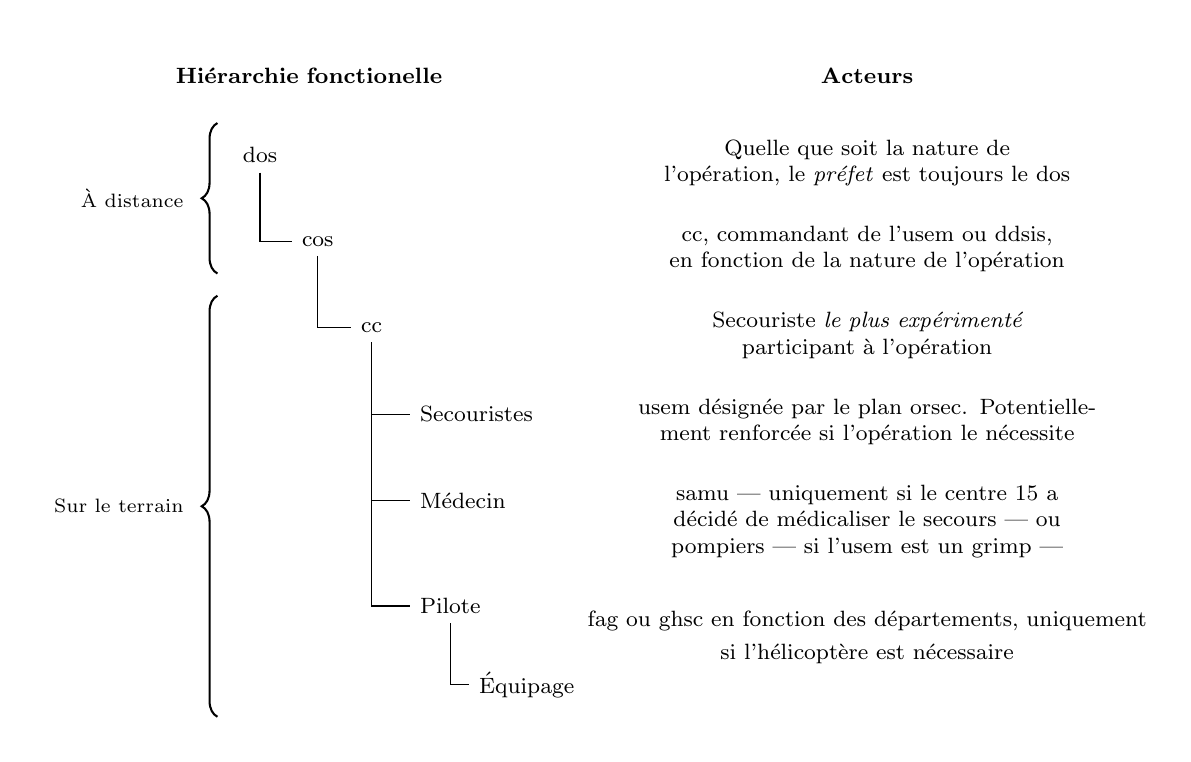
\begin{tikzpicture}
\usetikzlibrary{matrix, fit}
\usetikzlibrary{decorations.pathreplacing, calc}

\tikzset{ 
  table/.style={
    matrix of nodes,
    nodes={align=center, font=\footnotesize,  minimum height=10mm},
    nodes in empty cells,
    column 1/.style={nodes={text width=19em}},
    column 2/.style={nodes={text width=20em}}
  }
}

% Tableau
\matrix (m) [table] {
  % Ligne supérieure du tableau
  \toprule
  % Titre, en gras
  {\bfseries Hiérarchie fonctionelle} & {\bfseries Acteurs} \\
  \midrule
  % Pas de colonne 1, remplie après
  &Quelle que soit la nature de l'opération, le \emph{préfet} est
  toujours le \ac{dos}\\
  &\ac{cc}, commandant de l'\ac{usem} ou \ac{ddsis}, en fonction de
  la nature de l'opération\\
  &Secouriste \emph{le plus expérimenté} participant à l'opération\\
  &\ac{usem} désignée par le  plan \ac{orsec}. Potentiellement renforcée si l'opération le nécessite\\
  &\ac{samu} ---~uniquement si le centre 15 a décidé de médicaliser
  le secours~--- ou pompiers ---~si l'\ac{usem} est un
  \ac{grimp}~---\\
  % Lignes vides pour le multirow
  &\\
  &\\
};

% Texte centré sur les deux dernières lignes
\node[fit=(m-7-2)(m-8-2)]{\footnotesize \ac{fag} ou \ac{ghsc} en
  fonction des départements, uniquement si l'hélicoptère est
  nécessaire};
  
% Génération de l'arbre en colonne 1
\node[anchor=west](dos) at
([xshift=2.5cm]m-2-1.west){\footnotesize\ac{dos}};
%
\node[anchor=west](cos) at ([xshift=3.25cm]m-3-1.west)
{\footnotesize\ac{cos}};
%
\node[anchor=west](cc) at ([xshift=4cm]m-4-1.west)
{\footnotesize\ac{cc}};
%
\node[anchor=west](sec) at ([xshift=4.75cm]m-5-1.west)
{\footnotesize Secouristes};
%
\node[anchor=west](med) at ([xshift=4.75cm]m-6-1.west) {\footnotesize
  Médecin};
%
\node[anchor=west](heli) at ([xshift=4.75cm]m-7-1.west) {\footnotesize
  Pilote};
% 
\node[anchor=west](equi) at ([xshift=5.5cm]m-8-1.west) {\footnotesize
  Équipage};
% Arcs de l'arbre
\path[draw] (dos) |- (cos);
\path[draw] (cos) |- (cc);
\path[draw] (cc) |- (sec);
\path[draw] (cc) |- (med);
\path[draw] (cc) |- (heli);
\path[draw] (heli) |- (equi);

% Accolades
\draw [decorate,decoration={brace,amplitude=.2cm,
  raise=.2cm,mirror},line width=.75pt]
([xshift=2.5cm,yshift=-.1cm]m-2-1.north west) --
([xshift=2.5cm,yshift=.1cm]m-3-1.south west) node[midway, left,
xshift=-.5cm] {\scriptsize À distance};
%
\draw [decorate,decoration={brace,amplitude=.2cm,
  raise=.2cm,mirror},line width=.75pt]
([xshift=2.5cm,yshift=-.1cm]m-4-1.north west) --
([xshift=2.5cm,yshift=.1cm]m-8-1.south west) node[midway, left,
xshift=-.5cm] {\scriptsize Sur le terrain};
\end{tikzpicture}